\documentclass{beamer}

\usepackage{ucs}
\usepackage[utf8x]{inputenc}
\usepackage[T1]{fontenc}
\usepackage[english]{babel}
\usepackage[retainorgcmds]{IEEEtrantools}%	IEEEeqnarray
\usepackage{mathabx}%	convolution symbol
\usepackage{multi row}
\usepackage{epstopdf}
\usepackage{listings}


%	presentation info
\title{Scalability Problems In Shared Memory}

\author{José Alves, Rui Brito}

\institute[pg22765, pg22781]{
	Universidade do Minho
}

\date{Braga, March 2013}


%	beamer options
\usetheme{Frankfurt}


\begin{document}%	begin presentation

\maketitle%	title slide

\begin{frame}
	\frametitle{Index}
	\tableofcontents
\end{frame}


\section{Memory Bandwidth and Computational Intensity}
\subsection{}
\small
\begin{frame}
\begin{block}{Memory Bandwith}
	$Mem\_bandwidth = ((PAPI\_L2\_TCM) \times 64 \times 1 \times 10{-9}) / exec\_time$
	$measured\_mem\_bandwidth = (8427602 \times 64 \times 1 \times 10^{-9})/0.88 = 0.6129 GB/s$\\
	$System\_memory\_avail\_bandwidth = 14.8473 GB/s$
\end{block}
As seen in the December presentation, conv-diff has some locality problems (has it can also be seen by the high number of L1 misses (14937146)).
\end{frame}

\subsection{}
\begin{frame}[fragile]
		\begin{figure}[!htb]
			\centering
			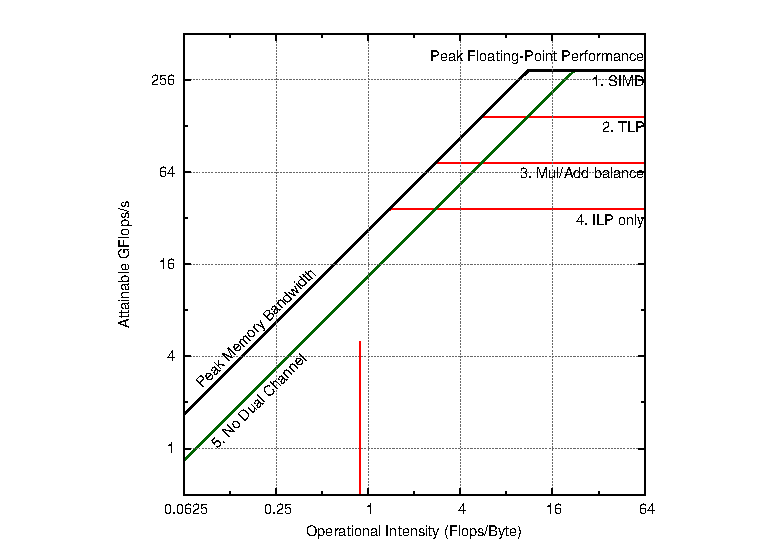
\includegraphics[scale=.7]{roofline_mbp.eps}
			\caption{Roofline for rMBP and conv\_diff}
			\label{roofline}
		\end{figure}
\end{frame}


\section{Measure Task Granularity}

\begin{frame}[fragile]
	\begin{block}{Task Granularity}
		In conv\_diff:									
		\begin{itemize}
			\item Only two parallel pieces of code run in parallel
			\item Large chunks of code
			\item Thread creation overhead is thus minimized 
		\end{itemize}
	\end{block}
\end{frame}

\section{Measure Programs Without Synchronisation}

\begin{frame}[fragile]

	{conv}\_diff is unsuitable for this sort of optimization:
	\begin{block}{Excessive task synchronization}		
		\begin{itemize}
			\item Reduction can't be used because values are updated in an array of pointers
			\item Synchronization must be forced on attributions
		\end{itemize}
	\end{block}
\end{frame}

\section{Measure Loads Per Task}

\begin{frame}[fragile]
	
	\begin{block}{Loads Per Task}
		\begin{itemize}
			\item Slight improvement using dynamic and guided scheduling
			\item Workload distribution also isn't the biggest problem
		\end{itemize}
	\end{block}

\end{frame}

\section{Conclusion}

\begin{frame}[fragile]
	
	\begin{block}{Conclusion}
		\begin{itemize}
			\item Bad data locality hinders the entire application performance
			\item Implementation either AoS or SoA is expected to improve performance drammaticaly 
			\item High chance that locality problem hides other problems
			\item Maybe what is not a problem now will prove to be so in the near future
		\end{itemize}
	\end{block}

\end{frame}

\end{document}%	end presentation